\subsection{Barrelfish}
\label{subsec:Barrelfish}
%<Kritika>
Barrelfish is a research operating system built by ETH Zurich and Microsoft Research, Cambridge.\footnote{http://www.barrelfish.org/} \footnote{http://research.microsoft.com/en-us/projects/barrelfish/} The motivation for building this system from scratch is to provide an OS for multi-core, many-core systems. Their aim is to support the scalability and the heterogeneous architecture that is sought after in current systems. 

A detailed review of the resource management for such a multi-core, heterogeneous system is provided in the works of Nevill et al. \cite{nevillmasters}. Nevill et al. analyse the capability management in such a system and specifically look at a single design for implementing it. If such systems have memory that is not shared or non-coherent memory, it requires that there be a separate kernel on each core in order to ensure that systems can manage and share resources. To do this there are various communication systems that it uses to synchronize the data between all the kernels and establish shared resources. 

Barrelfish capability design is based on the design of L4, and it is an extension of L4 in a multi-kernel system. The capability system for L4 is in fact the design for Barrelfish on a single core. The capability types are hence an extended version on L4 as well. It uses a domain specific language to define these capability type, which can be found in the appendix in \cite{nevillmasters}. We now mention a few examples of how Barrelfish extends the L4 design.

\begin{enumerate}
\item \textbf{Main Memory:} The RAM type is the equivalent of L4's \textit{Untyped Memory} and as in L4, it can be split into smaller parts.
\item \textbf{Page Tables:} Instead of having a separate page handler, in Barrelfish, the faulting applications themselves can manipulate the available memories through capabilities. This renders problems of external paging insignificant.
\item \textbf{Device Memory:} Barrelfish also has \textit{DevFrame} and \textit{PhsyAddr} capabilities, which ensure that there are capabilities that can be mapped to RAM capabilities without requiring that the memory be zeroed before it being read so as to prevent data leakage.
\item \textbf{Kernel Interface:} This feature enables Barrelfish to partition its kernel. The kernel is divided into privileged space and user space. As seen in \ref{kernelpartition} the user level can access the privileged operations by invoking Kernel capabilities via certain system calls.
\end{enumerate}

\begin{figure}[h]
 \centering
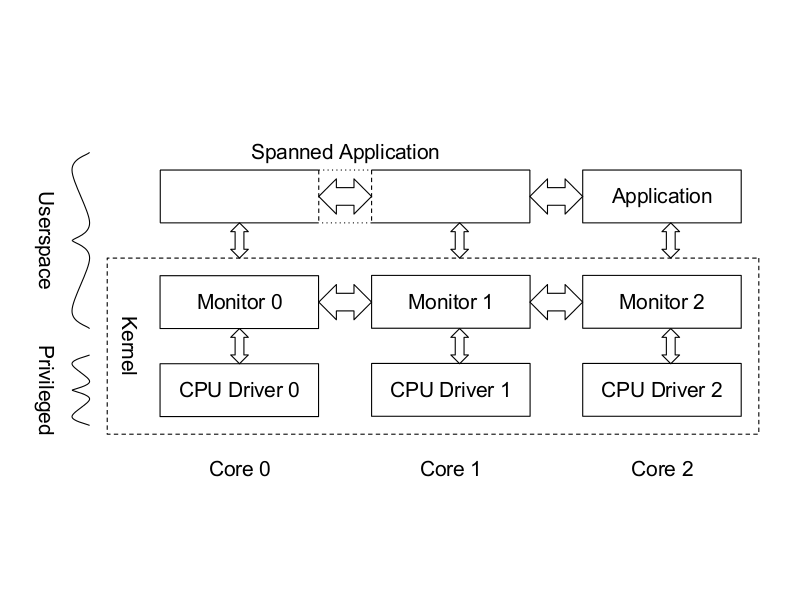
\includegraphics[scale=0.25]{img/BF_sharing_res}
\caption{Barrelfish Kernel Partitioning}
\label{kernelpartition}
\end{figure}
To manage resource utilization by the kernel, Barrelfish maintains an individual copy of the kernel on each core, and then performs synchronization to keep the system consistent. This is done to reduce the effort spent in synchronization, since the individual  copies have share-nothing policy by default. This design when extended to the userspace, creates a distributed system. This lets the system achieve the goal of running kernels on cores of different architectures in parallel. But it still faces the problems of low throughput and latency. The solution for this problem is to have a shared memory which does cache coherency, which requires certain communication channel between the cores to pass the capability information around. 

In \cite{nevillmasters}, the authors have presented basic operations that can be performed to when sharing of capability information is considered. The channels betweens cores maintain a send-once FIFO queue for sending messages containing these operations. Since sending and receiving these messages implies that there would be a need for synchronization between cores, there is a conflict which arises due to the fact that the initial goal was to maintain a synchronization-free system. The authors address this issue by considering object loyalty, which is that every capability object is assigned to an owning core. This ownership model is implemented along with certain defined invariants regarding the capability objects. \cite{nevillmasters} also gives preconditions and postconditions that must be met (as far as possible), to implement the Barrelfish capability operations.

We give a brief overview of the invariants, preconditions and postconditions below as mentioned in \cite{nevillmasters}-

\begin{enumerate}
\item \textbf{Invariants:}
	\begin{itemize}
	\item \textbf{Ownership Property:} Every capability that is not Null has an \textit{owner} property that refers to a running kernel instance in the system.
	\item \textbf{Consistent Ownership:} Any two capabilities that are copies must have the same \textit{owner} property.
	\item \textbf{Owner Copies:} Every set of all copies of a capability must contain at least one capability where the owner matches the location. With other words, the owning core must always have a local copy.
	\end{itemize}
	
\item \textbf{Preconditions:}
\begin{itemize}
\item \textbf{Copy:} The source capability is not Null and the destination core is valid.
\item \textbf{Retype:} The source capability is not Null, may be retyped to the destination type, and has no descendants in the system.
\item \textbf{Delete:} The target capability is not Null.
\item \textbf{Revoke:} The target capability is not Null.
\end{itemize}

\item \textbf{Postcondition:}
\begin{itemize}
\item \textbf{Copy:} The destination core has a copy of the capability and the invariants of the system hold.
\item \textbf{Retype:} The specified descendants exist in the target slots and the invariants of the system hold.
\item \textbf{Delete:} The source capability is Null and the invariants of the system hold.
\item \textbf{Revoke:} All copies and descendants of the source capability have been deleted and the invariants of the system hold.
\end{itemize}
\end{enumerate}

These operations all refer to slots of memory. A slot is the storage required to store an individual capability, where a Null capability corresponds to n empty slot. As mentioned above, every slot has an owner as well as an immutable memory location. The slots are considered local if the owner and the memory location are the same, and foreign otherwise. The behaviour and interaction between these capability operations are described through global pseudocodes (for each operation), which we will not mention here due to lack of space.

Barrelfish design has successfully applied aspects from an object oriented approach to a distributed, multi-core, many-core system. Though the authors have set out various optimizations as future scope and there are currently issues in the design regarding undelivered/ unresponsive messages, it does lay out the basic groundwork for other capability based resource management systems  to build on.